\documentclass[a4paper,14pt]{article}

\usepackage{comment} % Para comentar várias linhas ao mesmo tempo

%matemática
\usepackage{amsmath}
\usepackage{amssymb}

%diagramação
\usepackage{extsizes}
\everymath{\displaystyle}
\usepackage{geometry}
\usepackage{fancyhdr}
\usepackage{multicol}
\usepackage{graphicx}
\usepackage[brazil]{babel}
\usepackage[shortlabels]{enumitem}
\usepackage{cancel}
\usepackage{textcomp}
\usepackage{tcolorbox}

%tabelas
\usepackage{array} % Para melhor formatação de tabelas
\usepackage{longtable}
\usepackage{booktabs}  % Para linhas horizontais mais bonitas
\usepackage{float}   % Para usar o modificador [H]
\usepackage{caption} % Para usar legendas em tabelas
\usepackage{wrapfig} % Para usar tabelas e figuras flutuantes
\usepackage{xcolor} % Para cores do fundo de tabelas
\usepackage{colortbl} % Para cores do fundo de tabelas

%tikzpicture
\begin{comment}
	\usepackage{tikz}
	\usepackage{scalerel}
	\usepackage{pict2e}
	\usepackage{tkz-euclide}
	\usetikzlibrary{calc}
	\usetikzlibrary{patterns,arrows.meta}
	\usetikzlibrary{shadows}
	\usetikzlibrary{external}
\end{comment}


%pgfplots
\usepackage{pgfplots}
\pgfplotsset{compat=newest}
\usepgfplotslibrary{statistics}
\usepgfplotslibrary{fillbetween}

%colours
\usepackage{xcolor}



\columnsep=2cm
\hoffset=0cm
\textwidth=8cm
\setlength{\columnseprule}{.1pt}
\setlength{\columnsep}{2cm}
\renewcommand{\headrulewidth}{0pt}
\geometry{top=1in, bottom=1in, left=0.7in, right=0.5in}

\pagestyle{fancy}
\fancyhf{}
\fancyfoot[C]{\thepage}

\begin{document}
	
	\noindent\textbf{6FMA110 - Matemática} 
	
	\begin{center}Exercícios (II) (Versão estudante)
	\end{center}
	
	\noindent\textbf{Nome:} \underline{\hspace{10cm}}
	\noindent\textbf{Data:} \underline{\hspace{4cm}}
	
	%\section*{Questões de Matemática}
	
	\begin{multicols}{2}
		\begin{enumerate} 
			\item Na figura, $\Delta$$ABC \cong \Delta$$ABD$, \\~$m(A\hat{C}B) = 18$° e \\ $m(B\hat{A}D) = 46$°. Calcule a medida do menor ângulo $C\hat{B}D$.
			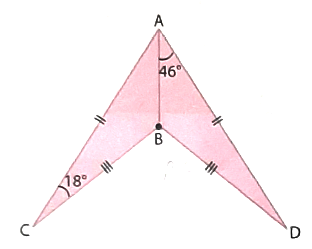
\includegraphics[width=1\linewidth]{6FMA110_imagens/imagem1}
			\\\\\\\\\\\\
			\item Dois triângulos com todos os ângulos iguais a 60° são sempre congruentes? Justifique. \\\\\\\\\\\\\\\\\\\\\\\\
			\item Na figura a seguir, \\ $\Delta$$ABC \cong \Delta$$ADC, AB = 5$ e \\ $BC = 7$. Calcule o perímetro do quadrilátero $ABCD$.
			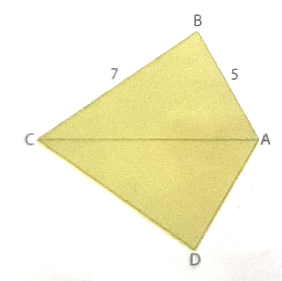
\includegraphics[width=1\linewidth]{6FMA110_imagens/imagem2} \\\\\\\\
			\item Na figura, temos $AB = 15, CF = 8, CD = 12, \Delta$$BCF \cong \Delta$$ECF$ e $\Delta$$ABF \cong \Delta$$DEC$. Sabendo que o $\Delta$$CFE$ é equilátero, calcule o perímetro do hexágono $ABCDEF$.
			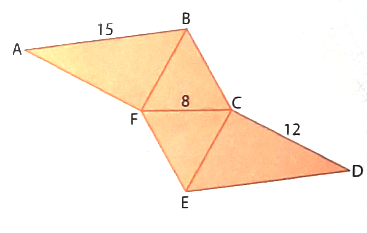
\includegraphics[width=1\linewidth]{6FMA110_imagens/imagem3} \newpage
			\textbf{Desafio olímpico} \\\\
			(OBMEP) Na figura, os pontos $A, B$ e $C$ estão alinhados. Qual é a soma dos ângulos marcados em cinza? \\
			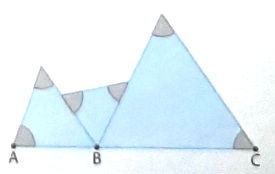
\includegraphics[width=1\linewidth]{6FMA110_imagens/imagem4}
			\begin{enumerate}[a)]
				\item 120°
				\item 180°
				\item 270°
				\item 360°
				\item 540° \newpage	
			\end{enumerate}
			\item Na figura a seguir; $\Delta$$ABD \cong \Delta$$CDB$,$~m(D\hat{A}B) = 24$° e $m(D\hat{B}C) = 20$°. Calcule a medida do ângulo $A\hat{B}C$. \\ 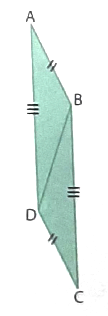
\includegraphics[width=0.5\linewidth]{6FMA110_imagens/imagem5}
			 \\\\\\\\\\\\\\\\\\\\\\\\\\\\\\\\\\\\\\
			\item Na figura a seguir, sabe-se que $\Delta$$AMB \cong \Delta$$AMD$ e $\Delta$$CMB \cong \Delta$$CMD$. Se $AB = 13, BC = 37, BD = 24$ e $AM = 5$, calcule os perímetros do quadrilátero $ABCD$ e do triângulo $AMD$.
			\textbf{Observação:}~$M$ é o ponto de intersecção dos segmentos $\overline{AC}$ e $\overline{BD}$ e $BM = MD$. \\ 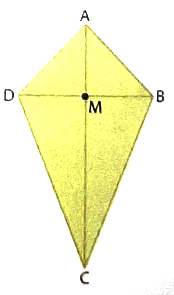
\includegraphics[width=0.7\linewidth]{6FMA110_imagens/imagem6} \newpage
			\item Na figura a seguir, os triângulos $ABD$ e $CBD$ são congruentes, $AD = 7$ e $AB = 6$. Determine o perímetro do quadrilátero $ABCD$. \\ 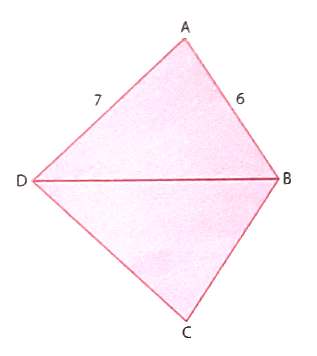
\includegraphics[width=1\linewidth]{6FMA110_imagens/imagem7} \columnbreak
			\item Na figura a seguir, $m(D\hat{B}C) = m(B\hat{C}D) = m(C\hat{D}B) = 60$°, $\Delta$$BCD \cong \Delta$$EAD$ e $AD = BD$. Calcule a medida do ângulo $E\hat{A}B$. 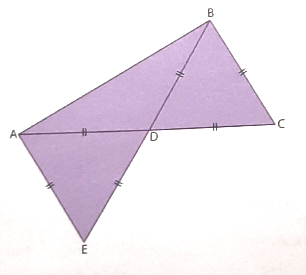
\includegraphics[width=1\linewidth]{6FMA110_imagens/imagem8} \newpage
			\item Na figura a seguir, $\Delta$$ADE \cong \Delta$$FBG$,~$m(F\hat{G}B) = 46$° e $BG = 2$. Determine as medidas do ângulo $C\hat{A}B$ e do segmento $\overline{DE}$ \\ 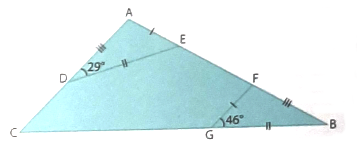
\includegraphics[width=1\linewidth]{6FMA110_imagens/imagem9}
		\end{enumerate}
		$~$ \\ $~$ \\ $~$ \\ $~$ \\	$~$ \\ $~$ \\ $~$ \\ $~$ \\ $~$ \\ $~$ \\ $~$ \\ $~$ \\ $~$ \\ $~$ \\ $~$ \\ $~$ \\ $~$ \\ $~$ \\ $~$ \\ $~$ \\ $~$ \\ $~$ \\ $~$ \\ $~$ \\ $~$ \\ $~$ \\ $~$ \\ $~$ \\ $~$ \\ $~$ \\ $~$ \\ $~$ \\ $~$ \\ $~$ \\ $~$ \\ $~$ \\ $~$ \\ $~$ \\ $~$ \\ $~$ \\ $~$ \\ $~$ \\ $~$ \\ $~$ \\ $~$ \\ $~$ \\ $~$ \\ $~$ \\ $~$ \\ $~$ \\ $~$ \\ $~$ \\ $~$ \\ $~$ \\ $~$ \\ $~$ \\ $~$ \\ $~$ \\ $~$ \\ $~$ \\ $~$ \\ $~$ \\ $~$ \\ $~$ \\ $~$ \\ $~$ \\ $~$ \\ $~$ \\ $~$ \\ $~$ \\ $~$ \\ $~$ \\ $~$ \\ $~$
	\end{multicols}
\end{document}